\documentclass{sciposter}
%\documentclass[a0,portrait]{sciposter}
%\documentclass[draft]{a0poster}
%\documentclass[portrait]{sciposter}
%\documentclass[a0paper,portrait]{sciposter}
%\documentclass[11pt, a4paper]{article}
\usepackage[utf8]{inputenc}  %%PC ou Unix

\usepackage{a0size}
\usepackage{amsmath}
\usepackage{amssymb}
\usepackage{multicol}
\usepackage[english]{babel}
\usepackage{setspace}
\usepackage[pdftex,final]{graphicx}
\graphicspath{Figures/}
\usepackage{epsfig}
\usepackage{dsfont}
\usepackage{bm}
\usepackage{pstricks,pst-grad}
\usepackage{color}
\usepackage{relsize}
\usepackage{url}
\usepackage{tikz}

\definecolor{BoxCol}{rgb}{0.2921,0.4921,0.7843}
\definecolor{SectionCol}{rgb}{1,1,1}
% uncomment for dark blue \section text 
\definecolor{TextColG}{rgb}{0,0.5,0}
\definecolor{TextColR}{rgb}{0.5,0,0}
\newcommand{\Rcolor}{\textcolor{TextColR}}
\newcommand{\Gcolor}{\textcolor{TextColG}}

%%%%%%%%%%%%%%%%%%%%%%%%%%%%%%%%
\renewcommand{\thesection}{\arabic{section}}
\newcommand{\sect}[1]{\setcounter{equation}{0}\section{#1}}
\renewcommand{\theequation}{\arabic{equation}} 
\newcommand{\seqna}{\begin{eqnarray}}
\newcommand{\eeqna}{\end{eqnarray}}
  
\newcounter{Theo}[section]  %\setcounter{noEx}{1}  
\def\theTheo{\arabic{Theo} de la section \thesection}
\def\numeroTheo{\arabic{Theo}}
\newenvironment{Theo}[1]{\vspace{-\lastskip}\vspace{1em}
\refstepcounter{Theo}\noindent{\bf Th\'eor\`eme \numeroTheo. #1}
\endgraf \leftskip1em{\parskip0pt\noindent}\ignorespaces
}{\par\vspace{1pt}}

\newcounter{Lemme}[section]  %\setcounter{noEx}{1}  
\def\theLemme{\arabic{Lemme} de la section \thesection}
\def\numeroLemme{\arabic{Lemme}}
\newenvironment{Lemme}[1]{\vspace{-\lastskip}\vspace{1em}
\refstepcounter{Lemme}\noindent{\bf Lemme \numeroLemme. #1}
\endgraf \leftskip1em{\parskip0pt\noindent}\ignorespaces
}{\par\vspace{1pt}}

\newcounter{Corollaire}[section]  %\setcounter{noEx}{1}  
\def\theCorollaire{\arabic{Corollaire} de la section \thesection}
\def\numeroCorollaire{\arabic{Corollaire}}
\newenvironment{Corollaire}[1]{\vspace{-\lastskip}\vspace{1em}
\refstepcounter{Corollaire}\noindent{\bf Corollaire \numeroCorollaire. #1}
\endgraf \leftskip1em{\parskip0pt\noindent}\ignorespaces
}{\par\vspace{1pt}}

%%%%%%%%%%%%%%%%%%%%%%%%%%
\let\bb\mathbb
\def \R {\mathbb{R}}
\def \N {\mathbb{N}}
\def \T {\mathbb{T}}
\def \L {\mathbb{L}}
\def \Z{\mathbb{Z}}
 
\def\gint{\displaystyle\int}
\def\gsum{\displaystyle\sum\limits}

%-------------------------------------------------------------------------------------------------------
\title{\begin{Huge}
Numerical approximation of propagation problems on the sphere using a compact scheme
\end{Huge}}
%\smallskip
\institute{{\bfseries M. Brachet, J.-P. Croisille}\hspace{9.5 in}  \\\hspace{0.5 in}
Institut Elie Cartan de Lorraine,  Université de Lorraine\hspace{1 in}\\\hspace{0 in}
B.P. 70239, F-54506 Vandoeuvre-lès-Nancy Cedex, France\hspace{6.5 in}\\}
\email{\hspace{1 in}  matthieu.brachet@univ-lorraine.fr\hspace{0.1 in}  }
% The following commands can be used to alter the default logo settings
\leftlogo[1.1]{LogoFNM}  % defines logo to left of title (with scale factor)
\rightlogo[1.4]{unicaen3}   % same but on right
%-------------------------------------------------------------------------------------------------------
\begin{document}
\conference{VI$^{\mbox{e}}$ Colloque EDP-Normandie, Caen 2017}
\maketitle


\vspace{0.5 cm}

%\vskip-1.5cm
\section*{Introduction}
Les équations Shallow Water \eqref{eq:SWEC} constituent le modèle de base pour la dynamique atmosphérique. Comme dans le cas de la dynamique des gaz (Equations d'Euler), la question est de disposer d'un schéma de haute précision en espace et en temps qui soit conservatif.
En climatologie mathématique, ce sont non seulement les quantités primaires (masse et quantité de mouvement) qui sont conservées mais également les quantités secondaires telles que l'énergie et l'enstrophie potentielle.

Notre approche est basée sur un schéma aux différences finies compact sur la grille Cubed-Sphere. Celui-ci est fortement relié aux méthodes en aéroacoustique numérique.

Des résultats numériques sont présentés, prouvant la pertinence de notre approche.

\begin{equation}
\label{eq:SWEC}
\left\lbrace
\begin{array}{rcl}
\dfrac{\partial \mathbf{u}}{\partial t} + \mathbf{u} \cdot \nabla_T \mathbf{u} + g \nabla_{T} h + f \mathbf{k} \wedge \mathbf{u} & = & \mathbf{0} \\
\dfrac{\partial h}{\partial t} + \nabla_T \cdot \left( h \mathbf{u} \right) & = & 0
\end{array}
\right.\text{  pour tout } \mathbf{x} \in \mathbb{S}_a^2 \text{ et } t>0.
\end{equation}

La notation $\nabla_T$ indique que l'opérateur est tangentiel.

\vskip1cm
\begin{multicols}{3} 

\section*{Cubed-Sphere}

La sphère est recouverte de 6 \textbf{panels} délimités par 6 grands cercles chacuns.

Le panel I est délimité par les 4 grands cercles :
\begin{itemize}
\item $C_V^1 = Vect(\mathbf{i}-\mathbf{j}, \mathbf{k}) \cap \mathbb{S}_a^2$,
\item $C_V^2 = Vect(\mathbf{i}+\mathbf{j}, \mathbf{k}) \cap \mathbb{S}_a^2$, il s'agit d'une rotation de $C_V^1$ d'un angle de $\pi/2$ autour de $(Oz)$,
\item $C_{II}^1 = Vect(\mathbf{i}+\mathbf{k}, \mathbf{j}) \cap \mathbb{S}_a^2$,
\item $C_{II}^2 = Vect(\mathbf{i}-\mathbf{k}, \mathbf{j}) \cap \mathbb{S}_a^2$, $C_{II}^2$ est une rotation de $C_{II}^1$ d'un angle de $\pi/2$ autour de $(Oy)$,.
\end{itemize}

\begin{figure}
\begin{center}
\includegraphics[scale=.83]{CS2.png}
\caption{La Cubed-Sphere.}
\end{center}
\end{figure}

Pour le panel I, on note 
\begin{itemize}
\item $C_i^{(1)}$ pour $-N/2 \leq i \leq N/2$ un ensemble de grands cercles passant par $\mathbf{N}$ et $\mathbf{S}$,
\item $C_j^{(2)}$ pour $-N/2 \leq j \leq N/2$ un ensemble de grands cercles passant par $\mathbf{E}$ et $\mathbf{W}$.
\end{itemize} 

$\mathbf{x}_{i,j}$, un point d'un panel, est un point de la \textbf{Cubed-Sphere} si 

\begin{equation}
\mathbf{x}_{i,j} = C_i^{(1)} \cap C_j^{(2)}.
\end{equation}


\begin{figure}[htbp]
\begin{center}
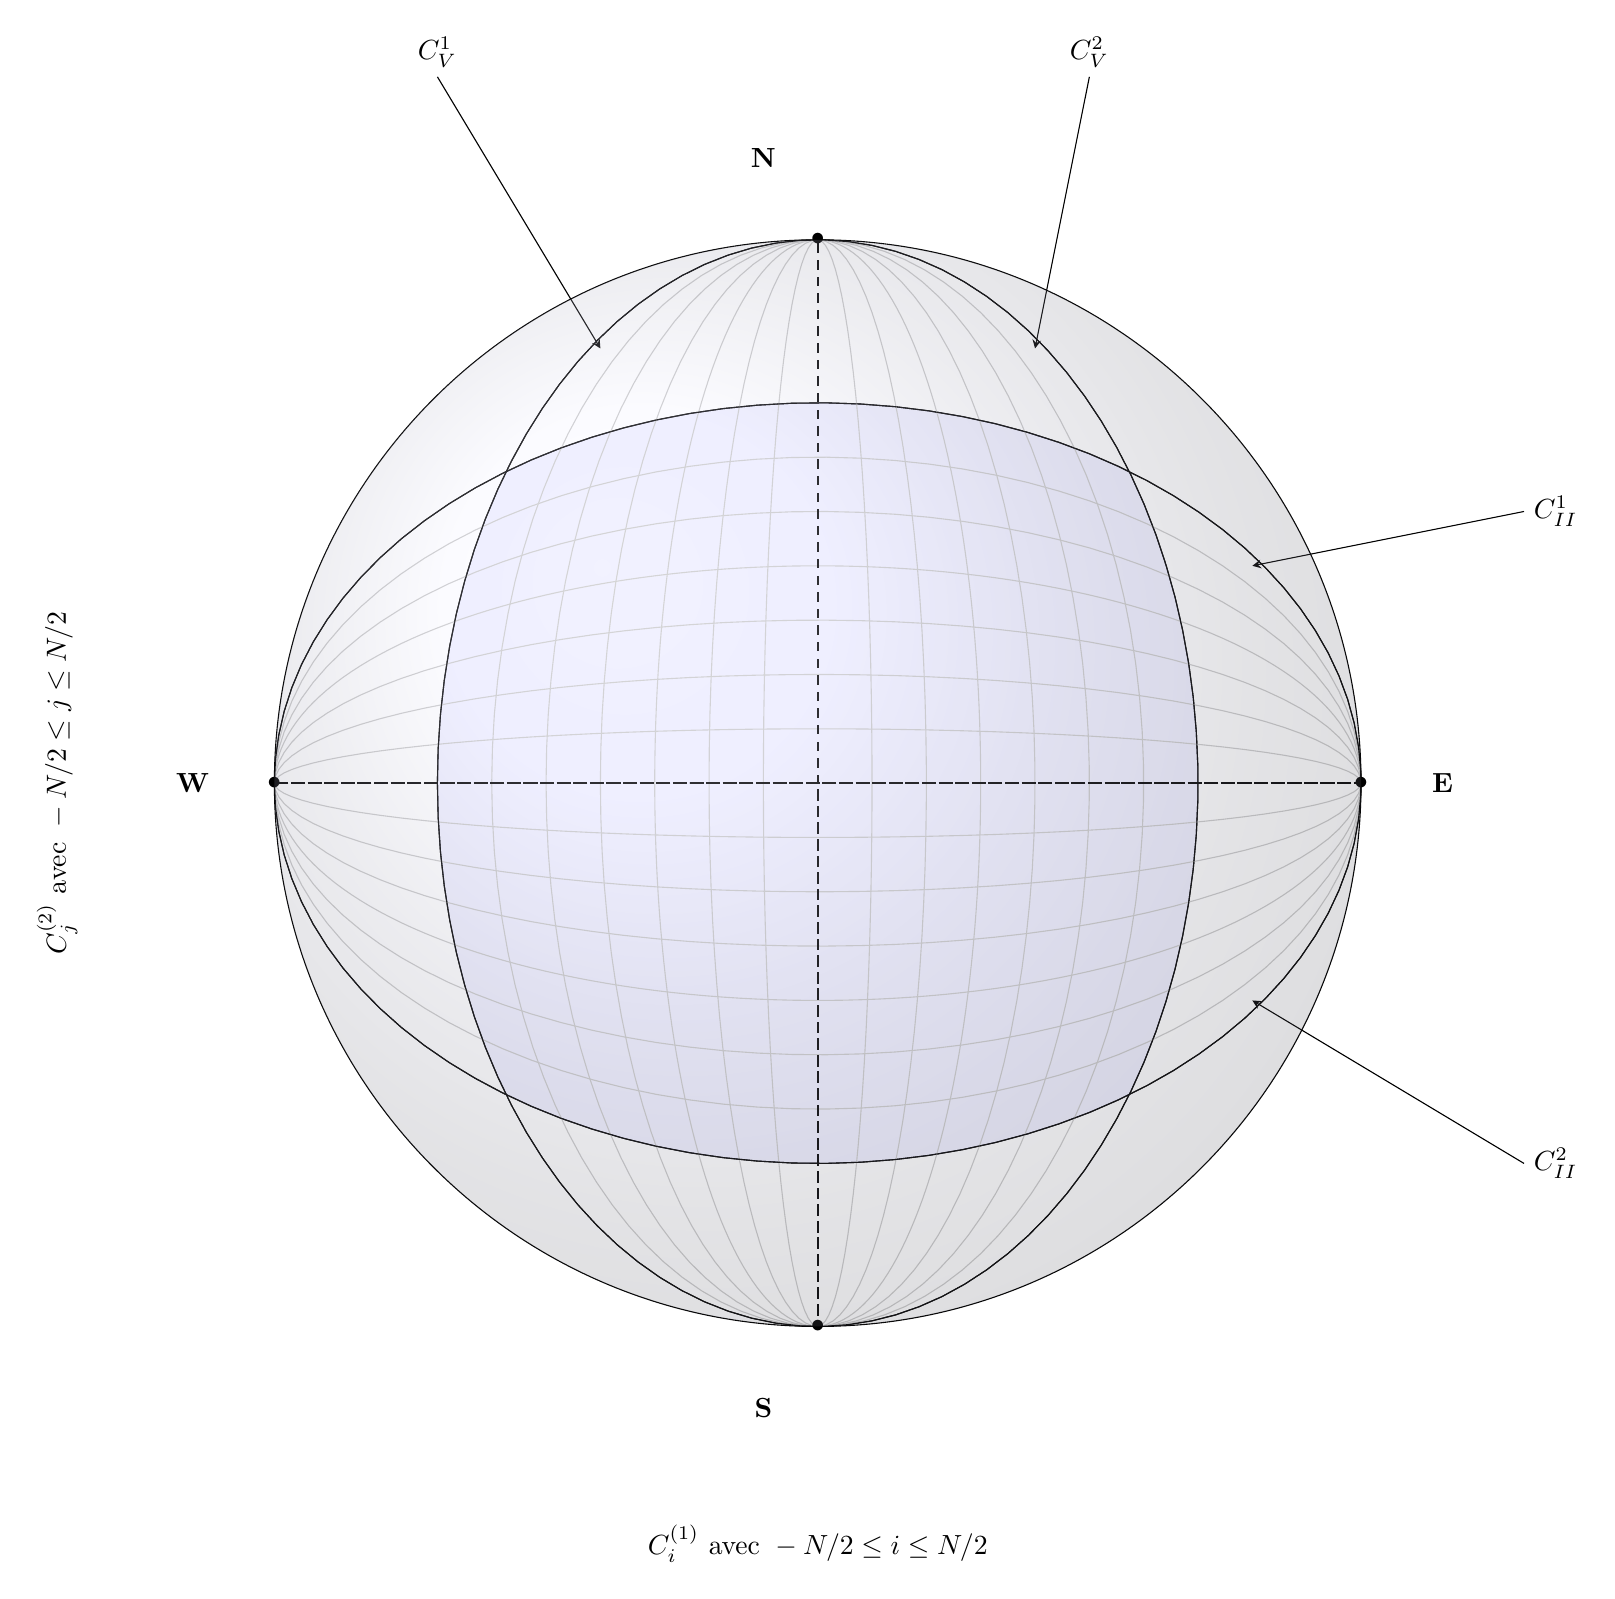
\begin{tikzpicture}[scale=6.9]
	%\draw [color=gray] (-1.5,-1.5) grid[step=0.1] (1.5,1.5);
	\draw [samples=100,domain=-180:180] plot({cos(\x)},{0.7*sin(\x)});
	\draw [samples=100,domain=180:-180] plot({0.7*cos(\x)},{sin(\x)}); 
	
	\filldraw[draw=black,fill=blue!30!white,opacity=0.20]
	plot [smooth,domain=-35:35] ({0.7*cos(\x)},{sin(\x)})
	-- plot [smooth,domain=55:125] ({cos(\x)},{0.7*sin(\x)})
	-- plot [smooth,domain=140:215] ({0.7*cos(\x)},{sin(\x)})
	-- plot [smooth,domain=230:305] ({cos(\x)},{0.7*sin(\x)})
	-- cycle;
	
	\draw [>=stealth, ->] (0.5,1.3) -- (0.4,0.8) ;
	\draw  (0.5,1.3) node[above] {$C_V^2$} ;
	\draw [>=stealth, ->] (-0.7,1.3) -- (-0.4,0.8) ;
	\draw  (-0.7,1.3) node[above] {$C_V^1$} ;
	\draw [>=stealth, ->] (1.3,0.5) -- (0.8,0.4) ;
	\draw  (1.3,0.5) node[right] {$C_{II}^1$} ;
	\draw [>=stealth, ->] (1.3,-0.7) -- (0.8,-0.4) ;
	\draw  (1.3,-0.7) node[right] {$C_{II}^2$} ;

	\draw [samples=100,domain=180:-180,color=gray!40] plot({cos(\x)},{0.1*sin(\x)});
	\draw [samples=100,domain=180:-180,color=gray!40] plot({cos(\x)},{0.2*sin(\x)});
	\draw [samples=100,domain=180:-180,color=gray!40] plot({cos(\x)},{0.3*sin(\x)});
	\draw [samples=100,domain=180:0,color=gray!40] plot({cos(\x)},{0.4*sin(\x)});
	\draw [samples=100,domain=0:-180,color=gray!40] plot({cos(\x)},{0.4*sin(\x)});
	\draw [samples=100,domain=180:-180,color=gray!40] plot({cos(\x)},{0.5*sin(\x)});
	\draw [samples=100,domain=180:-180,color=gray!40] plot({cos(\x)},{0.6*sin(\x)});
	\draw [samples=100,domain=180:-180,color=gray!40] plot({0.1*cos(\x)},{sin(\x)});
	\draw [samples=100,domain=180:-180,color=gray!40] plot({0.2*cos(\x)},{sin(\x)});
	\draw [samples=100,domain=-90:90,color=gray!40] plot({0.3*cos(\x)},{sin(\x)});
	\draw [samples=100,domain=90:270,color=gray!40] plot({0.3*cos(\x)},{sin(\x)});
	\draw [samples=100,domain=180:-180,color=gray!40] plot({0.4*cos(\x)},{sin(\x)});
	\draw [samples=100,domain=180:-180,color=gray!40] plot({0.5*cos(\x)},{sin(\x)});
	\draw [samples=100,domain=180:-180,color=gray!40] plot({0.6*cos(\x)},{sin(\x)});
	\draw [samples=100,domain=180:-180] plot({0.7*cos(\x)},{sin(\x)}); 
	\draw [dashed, line width=0.8pt, samples=100,domain=180:-180] plot({cos(\x)},{0*sin(\x)});
	\draw [samples=100,domain=180:-180] plot({cos(\x)},{0.7*sin(\x)});
	\draw [dashed, line width=0.8pt, samples=100,domain=180:-180] plot({0*cos(\x)},{sin(\x)});

	\draw  (0,1) node {$\bullet$} ;
	\draw  (-0.1,1.15) node {$\mathbf{N}$} ;
	\draw  (0,-1) node {$\bullet$} ;
	\draw  (-0.1,-1.15) node {$\mathbf{S}$} ;
	\draw  (1,0) node {$\bullet$} ;
	\draw  (1.15,0) node {$\mathbf{E}$} ;
	\draw  (-1,0) node {$\bullet$} ;
	\draw  (-1.15,0) node {$\mathbf{W}$} ;

%	\draw  (0.27,0.38) node {$\bullet$} ;
%	\draw  (0.27,0.38) node[right] {$\mathbf{x}$} ;
%	\draw [>=stealth, ->, color=blue] (0,-0.05) -- (0.3,-0.05) ;
%	\draw  (0.15,-0.05) node[color=blue, below] {$\xi$} ;
%	\draw [>=stealth, ->, color=red] (-.05,0) -- (-.05,0.4) ;
%	\draw  (-.05,0.2) node[color=red, left] {$\eta$} ;
    
    \draw  (-1.4,0) node[rotate=90] {$ C_j^{(2)}\text{ avec }-N/2\leq j \leq N/2$} ;
    \draw  (0,-1.4) node {$ C_i^{(1)}\text{ avec }-N/2\leq i \leq N/2$} ;
	
	\draw (0,0) circle (1cm);
    \shade[ball color=blue!10!white,opacity=0.20] (0,0) circle (1cm);
\end{tikzpicture}
\end{center}
\caption{Panel I}
\end{figure}

La discrétisation permet le calcul de \textbf{dérivées hermitiennes} le long des grands cercles. L'utilisation de grands cercles permets de travailler en contexte périodique et d'éviter les conditions de bords.

\vspace{1.89cm}

\section*{Approximation d'ordre 4 en espace et en temps}

Soit la fonction régulière 1-périodique
\begin{equation}
f : \mathbf{x} \in [0,1] \mapsto f(\mathbf{x}) \in \mathbb{R}
\end{equation}
On se donne $f_i = f(x_i)$ où $x_i = x_0 + i \Delta x$, $\Delta x=1/(N+1)$. $f$ est 1-périodique donc $f_0 = f_N$.

\begin{itemize}
\item Caclul d'\textbf{approximations hermitiennes d'ordre 4} :

on calcule $f_{x,i}$ l'approximation de $f'(x_i)$ :
\begin{equation}
\dfrac{1}{6} f_{x,i+1} + \dfrac{4}{6} f_{x,i} + \dfrac{1}{6} f_{x,i-1} = \dfrac{f_{i+1} - f_{i-1}}{2 \Delta x}
\end{equation}

\item \textbf{Filtrage} des hautes fréquences $\mathcal{F}$ :

\begin{equation}
\mathcal{F}(f)_i = \gsum_{m=0}^{5} a_m \left( f_{i+m} + f_{i-m} \right)
\end{equation}

avec 

\begin{equation}
\begin{bmatrix}
a_0\\a_1\\a_2\\a_3\\a_4\\a_5
\end{bmatrix} = 
\begin{bmatrix}
772/1024\\210/1024\\-120/1024\\45/1024\\-10/1024\\1/1024
\end{bmatrix}
\end{equation}

\begin{Theo}

Si $f \in \mathcal{C}^{10}$,
\begin{equation}
\mathcal{F}(f)_i - f(x_i) = \mathcal{O}(\Delta x^{10})
\end{equation}
\end{Theo}


\item Discrétisation en temps : méthode de \textbf{Runge-Kutta d'ordre 4} avec une étape de filtre à chaque pas de temps. On pose $q = [\mathbf{u},h]^T$.
\begin{equation}
\dfrac{dq}{dt} = F_{\nabla}(q)
\end{equation}

\begin{enumerate}
\item $K^{(1)} = F_{\nabla} \left( q^n \right)$,
\item $K^{(2)} = F_{\nabla} \left( q^n + \dfrac{\Delta t}{2} K^{(1)} \right)$,
\item $K^{(3)} = F_{\nabla} \left( q^n + \dfrac{\Delta t}{2} K^{(2)} \right)$,
\item $K^{(4)} = F_{\nabla} \left( q^n + \Delta t K^{(3)} \right)$,  
\item $q^{n+1} = \mathcal{F} \left( q^n  + \frac{\Delta t}{6} \left( K^{(1)} + 2 K^{(2)} + 2 K^{(3)} + K^{(4)} \right) \right)$.
\end{enumerate}
\end{itemize}

\section*{Analyse numérique}

On considère l'équation d'advection :
\begin{equation}
\left\lbrace
\begin{array}{rcl}
\dfrac{\partial h}{\partial t} + c \dfrac{\partial h}{\partial x} & = & 0 \\
h(t=0,x) & = & h_0(x)
\end{array}
\right. \text{ avec } x \in [0,1] \text{ et } t>0,
\label{eq:advection1D}
\end{equation}
dans un contexte périodique $h(t,x+1) = h(t,x)$ pour tous $t>0$ et $x \in [0,1]$.

Pour tout $1 \leq i \leq N$ et $n=0,1,...$, $h_i^n$ est une approximation de $h(t^n, x_i)$ obtenue avec le précédent schéma sur l'équation \eqref{eq:advection1D}. Par périodicité, on a $h_0^n = h_N^n$.

\begin{figure}[htbp]
\begin{center}
\begin{tikzpicture}[scale=3]
	\draw [>=stealth, <->] (-2,0.2) -- (-1,.2) ;
	\draw (-1.5,.3) node[above] {$\Delta x$} ;
	\draw (-3,0) -- (3,0) ;
	\draw (-3,0) node[color=yellow] {$\bullet$} ;
	\draw (-3,0) node {$\circ$} ;
	\draw (-3,-.2) node[below] {$x_0=0$} ;
	\draw (-2,0) node {$\bullet$} ;
	\draw (-2,-.2) node[below] {$x_1$} ;
	\draw (-1,0) node {$\bullet$} ;
	\draw (-1,-.2) node[below] {$x_2$} ;
	\draw (0,-.2) node[below] {$\ldots$} ;
	\draw (1,0) node {$\bullet$} ;
	\draw (1,-.2) node[below] {$x_{N-2}$} ;
	\draw (2,0) node {$\bullet$} ;
	\draw (2,-.2) node[below] {$x_{N-1}$} ;
	\draw (3,0) node[color=yellow] {$\bullet$} ;
	\draw (3,0) node {$\circ$} ;
	\draw (3,-.2) node[below] {$x_N =1$} ;
\end{tikzpicture}
\end{center}
\caption{Grille en dimension 1.}
\label{fig:maillage1D}
\end{figure}

\begin{Theo}

Sans filtre, le schéma est stable sous la condition CFL : 
\begin{equation}
\lambda = \dfrac{c \Delta t}{\Delta x} \leq \lambda_{\infty} = 2 \sqrt{\dfrac{2}{3}} \approx 1.6329
\end{equation}
\end{Theo}

Avec un filtre d'ordre $10$, le schéma est stable sous une meilleur condition $\lambda \leq \lambda_{10} \approx 1.6883$.

\begin{Theo}

Avec ou sans filtrage $\mathcal{F}$, le schéma est conservatif au sens où 
\begin{equation}
\forall n = 0,1,... \hspace{1cm} \Delta x \gsum_{i=1}^N h_i^{n+1} =  \Delta x \gsum_{i=1}^N h_i^{n}.
\end{equation}
\end{Theo}

\section*{Résultats numériques}

\begin{itemize}
\item \textbf{Test de J. Galewsky.} 
Le test de J. Galewsky est une perturbation d'une solution stationnaire. Ce test est difficile sur le maillage Cubed-Sphere.
\begin{itemize}
\item Fort gradient de $h$ sur le bord du panel V,
\item Perturbation initiale localisée au bord des panels I et V.
\end{itemize} 

\begin{figure}
\begin{center}
\includegraphics[scale=.73]{ref_7369437806_snapshot_intermediaire599.png}\\
\includegraphics[scale=.7]{ref_7369437806_massenergy.png}
\includegraphics[scale=.65]{ref_7369437806_enstrophy.png}
\end{center}
\caption{Vorticité au jour 6, erreurs relatives de conservations sur une grille $6 \times 128 \times 128$.}
\end{figure}

\item \textbf{Ondes de Rossby-Haurwitz.} Le test de Rossby-Haurwitz est un test classique de climatologie numérique. La condition initiale se déplace d'Ouest en Est.

\begin{figure}
\begin{center}
\includegraphics[scale=.73]{ref_7369145763_snapshot_intermediaire1399.png}\\
\includegraphics[scale=.65]{ref_7369145763_massenergy.png}
\includegraphics[scale=.65]{ref_7369145763_enstrophy.png}
\end{center}
\caption{$h$ au jour 14, erreurs relatives de conservations sur une grille $6 \times 80 \times 80$.}
\end{figure}
\end{itemize}


\section*{Perspectives}
\begin{itemize}
\item Etude en temps long des ondes de Rossby-Haurwitz,
\item Propriétés de conservations, quadrature numérique.
\end{itemize}



\bibliographystyle{plain}
\begin{thebibliography}{99}
\bibitem{BCyear} {\sc M. Brachet, J.-P. Croisille}, \textit{Numerical simulations of propagation problemes on the sphere
using a compact scheme}, soumis.
\end{thebibliography}
\end{multicols}








\end{document}
